% ============================================================================
%  Erasure is a Shift, Not a Deletion
%  Recovering Pretrained Semantics from Behavior-Cloned VLAs at Inference Time
%  arXiv-style paper (skeleton v0)
%  Author: Jatin Jani (Independent Researcher)
%  Template: kourgeorge/arxiv-style
% ============================================================================
\documentclass{article}

\usepackage{arxiv}
\usepackage[utf8]{inputenc}
\usepackage[T1]{fontenc}
\usepackage{hyperref}
\usepackage{url}
\usepackage{booktabs}
\usepackage{amsfonts}
\usepackage{amsmath}
\usepackage{nicefrac}
\usepackage{microtype}
\usepackage{float}
\setlength{\intextsep}{6pt plus 2pt minus 2pt}
\setlength{\floatsep}{8pt plus 2pt minus 2pt}
\setlength{\textfloatsep}{12pt plus 2pt minus 4pt}
\usepackage{cleveref}
\usepackage{graphicx}
\usepackage{natbib}
\usepackage{doi}
\usepackage{multirow}

\title{Erasure is a Shift, Not a Deletion: Recovering Pretrained Semantics from Behavior-Cloned VLAs at Inference Time}

\date{}

\newif\ifuniqueAffiliation
\uniqueAffiliationtrue

\ifuniqueAffiliation
\author{%
	Jatin Jani \\
	Independent Researcher\\
	\texttt{janijatin18@gmail.com} \\
}
\else
\usepackage{authblk}
\renewcommand\Authfont{\bfseries}
\setlength{\affilsep}{0em}
\author[1]{%
	Jatin Jani%
}
\affil[1]{Independent Researcher}
\fi

\renewcommand{\shorttitle}{Erasure is a Shift, Not a Deletion}

\hypersetup{
pdftitle={Erasure is a Shift, Not a Deletion: Recovering Pretrained Semantics from Behavior-Cloned VLAs at Inference Time},
pdfsubject={cs.RO, cs.LG, cs.CV},
pdfauthor={Jatin Jani},
pdfkeywords={Catastrophic Forgetting, Vision-Language-Action Models, Representation Alignment, Inference-Time Recovery, Foundation Model Adaptation, Robot Manipulation},
}

\begin{document}
\maketitle

% ============================================================================
% ABSTRACT (write last, current = draft spine)
% ============================================================================
\begin{abstract}
Behavior-cloning finetuning of a pretrained vision-language model (VLM) into a robot policy
erases the very semantics that made the VLM worth adapting: color grounding dies,
visual-reasoning accuracy drops by $86\%$ relative, and the backbone's representations
drift far from the pretrained geometry at the deepest layers. The field's response has been
to prevent this damage during training, on the implicit assumption that the erased knowledge
is destroyed. We show the assumption is false. On publicly released checkpoints (a
pretrained VLM, a behavior-cloned VLA, and an anchored VLA), we measure, with zero
training, that erasure is a \emph{shift, not a deletion}: the activations are displaced off
the pretrained manifold in a low-rank, deep-layer-concentrated way, measurable from the
checkpoint pair itself and correctable at inference. Adding the measured drift back at the
deep layers recovers a substantial fraction of the pretrained geometry (vision CKA $+15.4$
points), of the pretrained model's next-token behavior (logit agreement $+0.08$--$0.10$),
and of its exact answers under the restricted-answer GQA readout ($5.7\% \rightarrow 20.2\%$,
a $\times 3.5$ improvement), with a free-lunch regime in which action accuracy also
improves ($93\% \rightarrow 96\%$). The displacement is structured: a drift bundle of 32
principal directions per deep layer, roughly 1\,MB, recovers to within $0.8$ points of the
full-tensor correction on the shared evaluation set. We further show the mechanism behind the anchored
model's resistance: its frozen-head alignment objective is a manifold anchor, measured by a
transfer discriminator (the frozen head reads the anchored model's states at $90.0\%$
vs.\ $58.8\%$ for the behavior-cloned model's, through the same trained projection, while
the latter's information remains $89.9\%$ decodable). Three design principles follow for
foundation-model adaptation: (1) measure the drift before retraining, (2) ship drift bundles
with checkpoints, and (3) anchor or repair where the drift lives. The results also identify
a metric-level lesson: forgetting is visible to alignment-based readouts and invisible to
task-decodability probes. Code and logs that produced every number are released.
\end{abstract}

\keywords{Catastrophic Forgetting \and Vision-Language-Action Models \and Representation Alignment \and Inference-Time Recovery \and Foundation Model Adaptation \and Robot Manipulation \and Interpretability}

% ============================================================================
% 1. INTRODUCTION
% ============================================================================
\section{Introduction}
\label{sec:intro}

Vision-language-action (VLA) models are typically built by behavior-cloning finetuning: a
pretrained vision-language model (VLM) is adapted to expert demonstrations through supervised
action prediction, on the premise that finetuning transfers the VLM's semantic priors (its
understanding of color, shape, spatial layout, and language) into the resulting policy
\cite{brohan2022rt1,zitkovich2023rt2,driess2023palme,kim2024openvla,wang2025vlaadapter,starvla2026}.
The premise, however, is quietly broken. Behavior cloning progressively erases the very
semantics that made the VLM worth adapting. A policy finetuned to pick up a green mug reaches
for the green mug even when instructed to pick up the pink one. The backbone's
visual-reasoning accuracy on GQA \cite{hudson2019gqa} collapses by 86\% relative
($41.1\% \rightarrow 5.7\%$ in our measurements, while the source work reports a $94\%$ loss
under its own evaluation protocol \cite{dalal2026anchoralign}), and the finetuned backbone's
representations drift far from the pretrained geometry at the deepest layers (CKA
\cite{kornblith2019cka} to the pretrained VLM: $73.1\%$ for a behavior-cloned model vs.\
$97.0\%$ for a model trained with representation anchoring).

The field's response has been to prevent this damage during training: distillation and
feature-alignment losses toward the pretrained model
\cite{hinton2015distill,li2018lwf,mukhoti2024finetuning,kachaev2025donotblind}, co-training
on web image-text data \cite{zitkovich2023rt2,driess2023palme}, weight-space regularization
\cite{kirkpatrick2017ewc,huang2025maps}, and architectural anchors that freeze or shield
parts of the pretrained model
\cite{dalal2026anchoralign,driess2025knowledgeinsulation,grover2025preserving}. Every one of
these approaches implicitly assumes that the erased knowledge is gone, destroyed by the
action-supervision gradient, so the only defense is to stop the damage before it happens.

This paper asks the question that these approaches implicitly assume away: \emph{is the erased
knowledge actually destroyed?} On publicly released checkpoints, with zero training, we find
that it is not. Behavior-cloning finetuning does not delete pretrained semantics. It
\emph{displaces} them. The activations of the finetuned model sit off the pretrained manifold,
away from the fixed readout directions of the frozen pretrained language head, in a
displacement that is low-rank, concentrated in the deepest layers, and measurable directly
from the checkpoint pair itself.

If erasure is displacement, it should be correctable by moving the representations back. Across
six experiments on these artifacts (the pretrained VLM, a behavior-cloned VLA, and an
anchored VLA built on it), we show that it is:

\begin{itemize}
	\item \textbf{The drift is recoverable at inference.} Adding the measured drift back into
	the deep layers restores a substantial fraction of the pretrained geometry (vision CKA
	$+15.4$ points), of the pretrained model's next-token behavior (logit agreement
	$+0.08$--$0.10$), and of its exact answers (restricted-answer GQA accuracy
	$5.7\% \rightarrow 20.2\%$, a $\times 3.5$ improvement), with no training, no data, and
	no architectural change.
	\item \textbf{There is a free-lunch regime.} At small correction strength on the deepest
	layers, semantic alignment rises while action accuracy also improves ($93\% \rightarrow 96\%$).
	The semantics--control trade-off is real, but it is strength- and layer-controlled:
	deep-only correction dominates all-layer correction ($82\%$ vs.\ $41\%$ action accuracy).
	\item \textbf{The displacement is structured.} Thirty-two principal directions per deep
	layer reduce the drift's reconstruction error by $\approx 90\%$ and, as a drift bundle of
	roughly 1\,MB, recover to within $0.8$ points of the full-tensor correction, small
	enough for a checkpoint to ship.
	\item \textbf{The mechanism is identifiable.} The anchored model resists forgetting because
	its alignment objective routes supervision through the frozen pretrained language head,
	keeping its representations on the pretrained readout axes: the frozen head reads the
	anchored model's states at $90.0\%$ accuracy through the trained projection, versus
	$58.8\%$ for the behavior-cloned model's states through the same pathway, even though
	the behavior-cloned model's information remains linearly decodable at $89.9\%$.
\end{itemize}

Our contributions are: (1) we show that catastrophic forgetting in VLA
finetuning is a \emph{displacement, not a deletion}, measurable, structured, and recoverable
all the way to the pretrained model's exact answers; (2) we introduce \emph{displacement
correction}, inference-time recovery with zero training and no new data, including a documented
free-lunch regime and trade-off; (3) we introduce the \emph{drift bundle}, roughly 1\,MB of
principal directions that recover to within $0.8$ points of the full-tensor correction; (4) we provide a
mechanistic account of why frozen-head anchoring resists forgetting; and (5) we identify which
measurements reveal forgetting (representation-alignment and behavioral readouts) and which are
blind to it (task-decodability probes), a methodological distinction for evaluating adapted
foundation models.

All experiments use publicly released checkpoints and are measured at the readout level: the
representations, the pretrained model's next-token behavior, and its answers, the level at
which pretrained competence is defined. Carrying the results into closed-loop rollouts is a
natural next step. The evaluation protocol, per-experiment details, and the code and logs that
produced every number are released with the paper. Section~\ref{sec:related} positions this
work, Section~\ref{sec:setup} defines the testbed and the readout machinery,
Sections~\ref{sec:phenomenon}--\ref{sec:behavior} present the phenomenon, the recovery
mechanism, and the behavioral and answer-level evidence, Section~\ref{sec:principles} derives
design principles, and Section~\ref{sec:conclusion} concludes.

% ============================================================================
% 2. RELATED WORK
% ============================================================================
\section{Related Work}
\label{sec:related}

\textbf{Catastrophic forgetting in neural-network adaptation.} The observation that
finetuning overwrites pretrained knowledge is old \cite{kirkpatrick2017ewc,li2018lwf}.
The standard remedies regularize toward the pretrained model in weight space
\cite{kirkpatrick2017ewc,li2018lwf,douillard2020podnet} or distill its outputs
\cite{hinton2015distill,romero2015fitnets}. More recent work shows that finetuning can
quietly cripple a foundation model's features and argues for feature preservation
\cite{mukhoti2024finetuning}. This literature shares the implicit assumption that damage is
done at training time and can only be prevented there. We test that assumption directly and
find it false: the damage is a recoverable displacement, measurable from the checkpoint
pair and correctable at inference. The
observation that LoRA finetuning confines updates to a low-rank subspace
\cite{hu2022lora} is consistent with our structural findings, which make the consequence
explicit: the drift is low-rank, hence correctable with a small set of directions.

\textbf{Knowledge preservation in VLA finetuning.} VLA models adapt pretrained VLMs to
actions \cite{brohan2022rt1,zitkovich2023rt2,driess2023palme,kim2024openvla,
wang2025vlaadapter,starvla2026,black2025pi0}. Forgetting in this setting is typically
mitigated by co-training on web image-text data \cite{zitkovich2023rt2,driess2023palme},
by shielding the backbone from action gradients \cite{driess2025knowledgeinsulation}, by
module-wise proximity penalties \cite{huang2025maps}, by pairing a frozen vision encoder with
a trainable one \cite{grover2025preserving} or by aligning visual features to a frozen
foundation model \cite{kachaev2025donotblind}, or by anchoring the backbone to a frozen
copy of the pretrained VLM with layer-wise distillation and a frozen-head alignment loss
\cite{dalal2026anchoralign}. Our paper uses the released checkpoints of the anchoring approach
\cite{dalal2026anchoralign} as an off-the-shelf testbed (Section~\ref{sec:artifacts}). Its subject is not the
training recipe but the nature of the erasure that recipe prevents.

\textbf{Representation alignment, readouts, and activation interventions.} Measuring how far
a finetuned model has drifted is standard practice via CKA \cite{kornblith2019cka}, and
linear probing quantifies what remains decodable. Interventions on activations at inference,
such as steering vectors and activation patching \cite{turner2023steering,li2023iti}, are
established instruments in interpretability, and we use them as the \emph{measurement instrument} for recoverability, with
the intervention direction derived from the checkpoint pair itself rather than from human
labels. To our knowledge, no prior work measures whether erased semantics in a finetuned
policy are recoverable at inference, structures the drift into a shippable bundle, or
demonstrates recovery of the pretrained model's exact answers.

% ============================================================================
% 3. SETUP
% ============================================================================
\section{Setup}
\label{sec:setup}

\subsection{Released artifacts as a public testbed}
\label{sec:artifacts}

All experiments use three publicly released checkpoints from the same architecture family: the
pretrained VLM (Prismatic-Qwen2.5-0.5B \cite{karamcheti2024prismatic,yang2024qwen25}, a
Qwen2.5-0.5B language model with fused DINOv2 \cite{oquab2024dinov2} and SigLIP
\cite{zhai2023siglip} vision encoders), a behavior-cloned VLA finetuned on the LIBERO-Spatial
suite (the released VLA-Adapter checkpoint \cite{wang2025vlaadapter}\footnote{The
behavior-cloned checkpoint we study is the officially released VLA-Adapter model, not a
baseline retrained for the source work. Absolute forgetting magnitudes may differ
accordingly, while the ordering between the two finetuned models is stable across every
frame set we evaluate (Table~\ref{tab:gate}).}), and an anchored VLA
trained with layer-wise distillation and frozen-head alignment against the pretrained VLM
(the released Anchor-Align checkpoint \cite{dalal2026anchoralign}). We also use the LIBERO-Spatial RLDS demonstrations
\cite{liu2023libero,oneill2024openx} as the frame source, and a GQA validation subset
\cite{hudson2019gqa} for the answer-level readouts of
Section~\ref{sec:gqa}. All three models share the same 896-dim hidden dimension. The two finetuned models
share the same LoRA-rank-64 finetuning regime \cite{hu2022lora} and input representation,
and differ only in the finetuning objective. We treat this triple as an off-the-shelf testbed:
the artifacts are the instruments of this paper, not its subject.

\subsection{Frozen-head readout machinery}
\label{sec:readout}

We measure the pretrained model's semantics through a \emph{frozen-head readout}: the frozen,
unmodified language-model head of the pretrained VLM, applied to the hidden state at the
\emph{answer position}, the last instruction or question token, i.e.\ the position
immediately before generation. Because this head is the decoder through which the pretrained
model itself expresses what it knows, readability through it measures how much of the
pretrained model's semantics the finetuned representation retains. The same frozen head is
applied to all three models, making it a fixed readout instrument. Inputs use the VLA prompt format
(\texttt{In: \{instruction\}\textbackslash nOut:}) and the same two-camera image stack for every
model, so differences in readout are attributable to the models' representations alone.

For open-form questions (Section~\ref{sec:gqa}) we use the standard restricted-answer
protocol: the readout is the argmax over the \emph{sampled answer vocabulary} of the dataset,
rather than over the full 151{,}636-token vocabulary, where the argmax is dominated by the
language prior. For measuring whether a finetuned model still \emph{behaves} like the pretrained
one (Section~\ref{sec:agreement}), we compare next-token logits against the pretrained
model's, using logit cosine, centered cosine, top-1 agreement, and top-5 agreement, all
label-free.

\subsection{Drift and displacement correction}
\label{sec:drift}

The \emph{drift} of a finetuned model is the per-layer, per-position activation difference
between it and the pretrained model, averaged over a set of training frames:
$\Delta^u[\mathrm{pos}] = \mathbb{E}_{\mathrm{frames}}\big[H^u_{\mathrm{base}}[\mathrm{pos}]
- H^u_{\mathrm{BC}}[\mathrm{pos}]\big]$, for each decoder layer $u$ and aligned position.
Position alignment follows the token layout. Vision tokens align by absolute index, text
tokens by offset from the answer position, and the action region is excluded because the
pretrained model has no action tokens. \emph{Displacement correction} injects $\alpha\cdot\Delta$ back at
inference time, into the finetuned model's forward pass at the chosen layers via
residual-stream hooks, with no training, no weight changes, and no extra data. The
coefficient $\alpha$ controls the correction strength. We also
consider (i) the \emph{drift bundle}, the rank-$k$ reconstruction
$\hat\Delta_k = U_k S_k V_k^{\top}$ obtained from the per-layer singular value decomposition of
$\Delta$ (Section~\ref{sec:structure}), and (ii) the \emph{per-sample} correction, each frame's
own $\Delta$, the least-approximated correction in our method family.

\subsection{Evaluation protocol}
\label{sec:protocol}

All measurements follow a same-frames protocol: every model is evaluated on identical inputs,
and every baseline--corrected pair is measured on the same frames. Evaluation frames are drawn from the demonstration distribution and shared across every condition, so all reported differences are paired comparisons on identical inputs. The semantic axes are
(1) representation alignment, measured as CKA \cite{kornblith2019cka} to the pretrained model
over text-tail and vision-token positions; (2) behavioral agreement, the frozen-head next-token
metrics above; and (3) answer accuracy, the restricted-answer GQA readout. Where correction
competes with the task objective, we also report action direction accuracy and the mean
chunk-level $\ell_2$ action error. Experiments E0--E5 (phenomenon, displacement correction,
drift structure, frozen-head readability, behavioral agreement, and answer recovery,
respectively) and their exact protocols, grids, and frame counts are detailed in
Appendix~\ref{app:protocols}. The code and logs that produced
every number in this paper are released.

% ============================================================================
% 4. PHENOMENON
% ============================================================================
\section{Phenomenon: deep-layer erasure of pretrained representations}
\label{sec:phenomenon}

We first establish the phenomenon on released artifacts: the behavior-cloned model's
representations have drifted far from the pretrained geometry, and the drift concentrates in
the deepest layers: the layers immediately before the frozen-head readout of the
model's next token. Figure~\ref{fig:cka} shows per-layer text-token CKA to the pretrained VLM
for the two finetuned models. The behavior-cloned model is nearly identical to the pretrained
one in early layers (embeddings and shallow LoRA adapters change little), then collapses
with depth: layer-24 CKA drops to $\approx 0.6$, with the steepest loss in
layers 21--24. The anchored model stays flat throughout ($\ge 0.93$ at every layer). Table~\ref{tab:gate}
shows that the deep-layer gap is stable across three independent frame sets
($24.5$ / $24.8$ / $23.9$ points).

The vision stream carries an even stronger signal: the behavior-cloned model's deep-layer
vision-token CKA to the pretrained VLM is $46.6\%$ (the number we later use to measure
recovery). The pattern is the same signature the source work documented in its own evaluation
\cite{dalal2026anchoralign}: forgetting is real, reproducible with released artifacts, and
preferentially destroys the deepest layers. Why the deepest layers? Because they are where
the action objective reaches in, and where the frozen readout decides behavior, the subject
of Section~\ref{sec:behavior}. Whether this apparent erasure has destroyed the pretrained
semantics or merely displaced them is the question the rest of the paper turns on.

\begin{figure}[t]
	\centering
	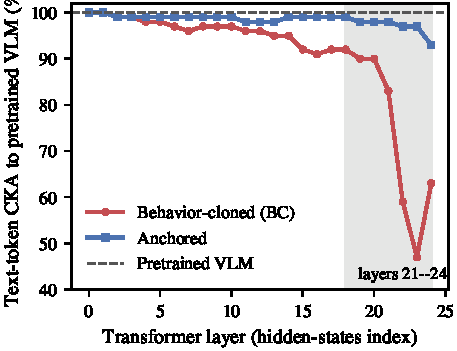
\includegraphics[width=0.65\linewidth]{figures/fig1_cka_curves.pdf}
	\caption{Per-layer text-token CKA to the pretrained VLM, for the behavior-cloned and the
	anchored model (release artifacts). The behavior-cloned model collapses in layers 21--24
	(layer-24 CKA $\approx 0.6$), while the anchored model stays flat ($\ge 0.93$ at every layer). Early
	layers are trivially identical (embeddings untouched).}
	\label{fig:cka}
\end{figure}

\begin{table}[t]
	\centering
	\caption{Deep-layer (layers 18--23) text-token CKA to the pretrained VLM, across three
	independent frame sets. The gap is stable (24.5 / 24.8 / 23.9 points).}
	\label{tab:gate}
	\begin{tabular}{lccc}
		\toprule
		& set 1 & set 2 & set 3 \\
		\midrule
		BC (behavior-cloned)   & 72.8\% & 72.1\% & 73.1\% \\
		Anchored               & 97.4\% & 96.9\% & 97.0\% \\
		\midrule
		gap                    & 24.5 & 24.8 & 23.9 \\
		\bottomrule
	\end{tabular}
\end{table}

% ============================================================================
% 5. MECHANISM: RECOVERY
% ============================================================================
\section{Mechanism I: erasure is displacement, not deletion}
\label{sec:recovery}

If erasure were deletion (information destroyed by the action-supervision gradient), no
post-hoc intervention could recover it. If erasure is displacement, the drift
$\Delta$ measured from the checkpoint pair quantifies that displacement, and adding it back
at inference should restore the pretrained geometry. The two hypotheses make opposite
predictions for a single intervention, and we run it directly.

\subsection{The recovery experiment}
\label{sec:rec-exp}

We compute $\Delta$ over a set of training frames, inject $\alpha\cdot\Delta$ into the
behavior-cloned model's deep layers via forward hooks, and measure semantic recovery
(CKA to the pretrained model) against action fidelity (action direction accuracy and mean
chunk-level $\ell_2$ error) on the shared evaluation set. Figure~\ref{fig:tradeoff} and
Table~\ref{tab:recovery} show the result. Correcting layers 18--23 at unit strength recovers
$15.4$ CKA points of the vision stream ($46.6\% \rightarrow 62.0\%$) and $7.1$ points at
layer 24 of the text stream. Deletion predicts that this intervention should do nothing.
Instead, the pretrained geometry returns along the measured drift, confirming the displacement
hypothesis. The correction is not free of tension with the task: at unit
strength, action direction accuracy falls from $93\%$ to $82\%$ and action error rises as
$\alpha$ increases. But the tension is confined and controlled by strength and layer choice.
As we show next, it vanishes entirely in a free-lunch regime.

\subsection{The free-lunch regime}
\label{sec:freelunch}

At small correction strength on the deepest layers ($\alpha = 0.25$ on layers 21--24),
the trade-off disappears: semantic alignment \emph{rises} (layer-24 text CKA
$90.4\% \rightarrow 96.8\%$) while action accuracy
\emph{improves} ($93\% \rightarrow 96\%$) and action error stays flat ($0.51$ vs.\ $0.51$).
Small deep-layer correction acts as a soft regularizer rather than a perturbation. The
practical reading is that the semantics--control trade-off commonly assumed to be fundamental
in VLA finetuning is, at least in this regime, an artifact of correcting too much, or
correcting in the wrong places. Correcting \emph{all} layers at unit strength collapses action
accuracy to $41\%$ (Table~\ref{tab:recovery}) and recovers no more semantic alignment than
deep-only correction ($57.5\%$ vs.\ $62.0\%$ vision CKA), which retains $82\%$ of the action
accuracy: the displacement lives in the deep layers, and that is where correction belongs.

\subsection{Controls: the correction is directional}
\label{sec:controls}

Three controls establish that the recovery is attributable to the drift's content, not to the
perturbation itself. (i) \emph{Random directions:} replacing $\Delta$ with norm-matched random
directions does not recover alignment. It \emph{hurts} it (deep-layer text CKA drops from the
$95.2\%$ baseline to $87.6\%$). Magnitude alone explains nothing. The direction of $\Delta$
carries the semantics. (ii) \emph{Reverse correction:} applying $-\Delta$ to the pretrained
model lands it at the behavior-cloned model's alignment (deep-layer text CKA $94.1\%$ vs.\
$95.2\%$), confirming that $\Delta$ is the displacement axis training moved along. (iii)
\emph{Semantic axis:} pushing the anchored model along the same axis ($\Delta' =
\mathrm{anchored} - \mathrm{BC}$) degrades its preserved alignment toward the behavior-cloned
level ($97.0\% \rightarrow 92.9\%$), showing the drift axis is semantic rather than arbitrary.
Finally, the per-sample correction (each frame's own $\Delta$) recovers a substantial
fraction of the pretrained model's answers (Section~\ref{sec:gqa}).

\begin{figure}[t]
	\centering
	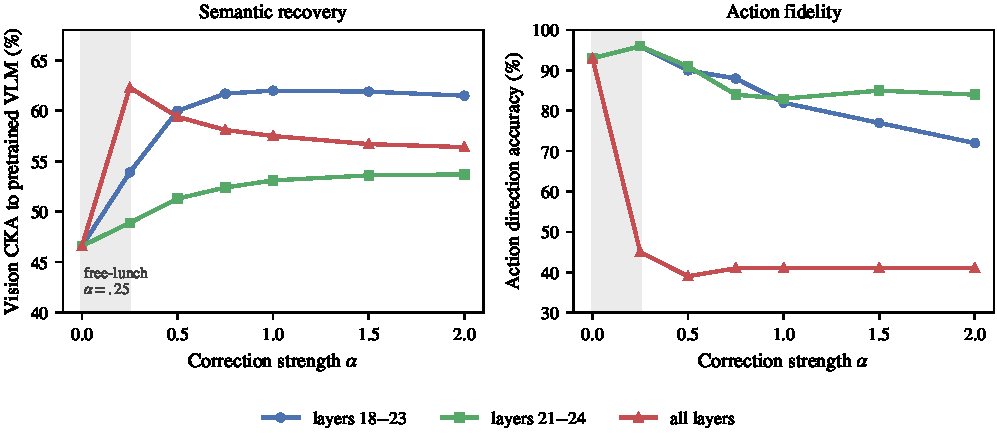
\includegraphics[width=\linewidth]{figures/fig2_tradeoff.pdf}
	\caption{Semantic recovery (vision CKA to base) vs.\ action fidelity (AP accuracy and
	chunk L2) as the correction strength $\alpha$ increases, for three layer subsets. A
	free-lunch region exists at small $\alpha$ on layers 21--24, while all-layer correction
	collapses actions.}
	\label{fig:tradeoff}
\end{figure}

\begin{table}[t]
	\centering
	\caption{Representative configurations of the displacement-correction sweep (100 shared evaluation
	frames). Deep-only correction recovers vision CKA while retaining actions, whereas all-layer
	correction destroys them and norm-matched random directions do not recover alignment.}
	\label{tab:recovery}
	\begin{tabular}{lccc}
		\toprule
		config & vis CKA & AP acc & L2 \\
		\midrule
		BC (no correction)          & 46.6\% & 93\% & 0.51 \\
		layers 21--24, $\alpha=.25$ & 48.9\% & 96\% & 0.51 \\
		layers 18--23, $\alpha=1.0$ & 62.0\% & 82\% & 1.93 \\
		all layers, $\alpha=1.0$    & 57.5\% & 41\% & 2.67 \\
		random directions           & 56.1\% & 90\% & 0.59 \\
		\bottomrule
	\end{tabular}
\end{table}

% ============================================================================
% 6. MECHANISM: DRIFT STRUCTURE
% ============================================================================
\section{Mechanism II: the drift is low-rank and bundle-able}
\label{sec:structure}

The recovery of Section~\ref{sec:recovery} uses the full per-position drift tensor. A
deployable method should not require it: if the displacement is structured, concentrated
in few directions and in the deep layers, then a small number of principal directions
should reproduce the correction. We test this with the singular value decomposition of
$\Delta$, per layer and per token region (vision and text tokens have distinct drift
statistics).

\textbf{The drift is low-rank.} Figure~\ref{fig:bundle} (left) shows the relative Frobenius
reconstruction error of the rank-$k$ approximation $\hat\Delta_k$, averaged over the deep
layers and both token regions. The error falls monotonically with $k$: a single direction
nearly halves it (to $53.95\%$), 8 directions remove $70\%$ of it, and 32 directions
reduce it by $\approx 90\%$ (to $9.98\%$ relative error).

\textbf{The bundle reproduces the correction.} Figure~\ref{fig:bundle} (right) shows the
semantic recovery obtained by patching with the rank-$k$ bundle instead of the full tensor,
at unit strength on the deep layers, evaluated on the shared evaluation set. The recovery curve saturates
quickly: the 8-direction bundle captures $77\%$ of the recoverable gain, and the
32-direction bundle attains $60.1\%$ vision CKA versus $60.9\%$ for the full tensor,
within $0.8$ points of the exact correction. In bfloat16, the bundle stores roughly $1$\,MB
for this model family, a $6.5\times$ compression of the dense deep-layer correction
($\approx 6$\,MB).

\textbf{The drift lives where the erasure happens.} The per-layer drift norm correlates
with the per-layer CKA collapse ($r = +0.67$): the layers with the largest displacement are
the layers where the pretrained geometry is most destroyed. The collapse and the drift point
at the same layers, which is why deep-only correction suffices
(Section~\ref{sec:recovery}).

\begin{figure}[t]
	\centering
	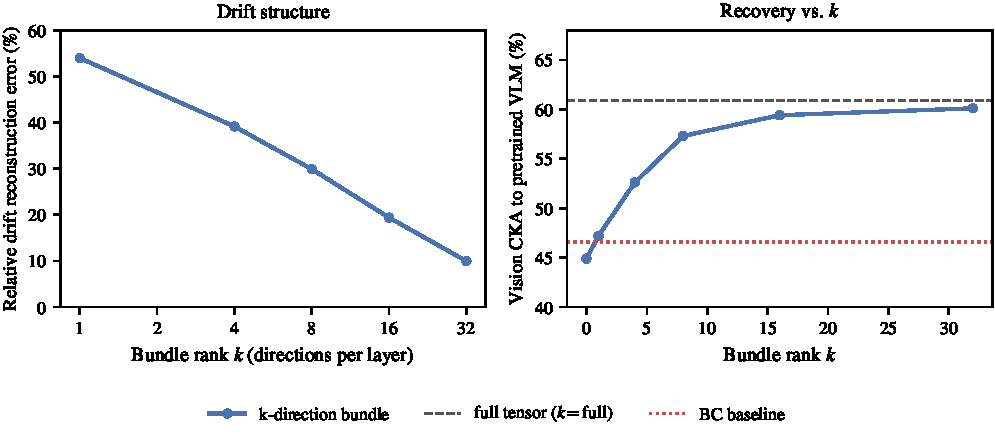
\includegraphics[width=\linewidth]{figures/fig3_bundle.pdf}
	\caption{Left: relative reconstruction error of the drift vs.\ the number of principal
	directions $k$ (32 directions $\approx$ 10\% error). Right: semantic recovery achieved by
	patching with the $k$-direction bundle ($k{=}32 \approx k{=}\text{full}$).}
	\label{fig:bundle}
\end{figure}

% ============================================================================
% 7. MECHANISM: FROZEN HEAD
% ============================================================================
\section{Mechanism III: the frozen head is a manifold anchor}
\label{sec:frozenhead}

Why does the anchored model resist forgetting at all? Its training objective pairs
distillation toward a frozen copy of the pretrained VLM with an alignment loss whose
gradient reaches the backbone only through a frozen pretrained language-model head via a
trained projection: the backbone can only reduce this loss by keeping the projected
representation readable through the frozen head's fixed directions. Our measurements
quantify the pathway and show the frozen head acting as a manifold anchor.

\textbf{The frozen head reads direction through the trained projection.} Motion-direction
words are decoded from the anchored model's answer-position states by the frozen head
together with its released trained projection, at $90.0\%$ accuracy, while with an identity
projection the same states read at $22.0\%$ (chance is $16.7\%$). The projection is what
maps the representation onto the frozen head's readout axes. It is the alignment loss's only
route to the backbone, and the mechanism by which frozen-head supervision ties the
representation to the pretrained head's readout axes.

\textbf{The transfer discriminator.} The same trained projection that reads the anchored
model's states at $90.0\%$ reads the behavior-cloned model's states at only $58.8\%$, a
gap of $31.2$ points (standard error $\approx 3.6$, $n = 250$). Yet the information is
present: a freshly fit linear probe recovers the behavior-cloned model's direction at
$89.9\%$. Because the projection is a fixed linear map, its deficit on the behavior-cloned
states cannot reflect missing information. What has moved is the readout geometry
itself. The behavior-cloned model's knowledge is intact and extractable, displaced off the
pretrained readout axes rather than lost. This is the paper's central claim in its most
direct form: erasure is a displacement of the readout geometry, not a loss of knowledge.
The displacement is graded rather than binary ($58.8\%$, not chance), consistent with the
moderate drift magnitude of Sections~\ref{sec:phenomenon}--\ref{sec:structure}: a partial
shift, not an axis swap.

\begin{figure}[t]
	\centering
	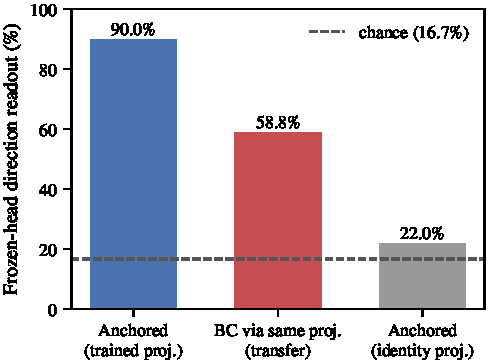
\includegraphics[width=0.65\linewidth]{figures/fig4_readability.pdf}
	\caption{Frozen-head readability of motion direction. The anchored model's states remain
	readable through its trained projection (90.0\%), while the behavior-cloned model's states
	are read at only 58.8\% by the same pathway, despite 89.9\% linear decodability.}
	\label{fig:readability}
\end{figure}

% ============================================================================
% 8. BEHAVIOR AND ANSWERS
% ============================================================================
\section{Behavioral erasure and the recovery of pretrained answers}
\label{sec:behavior}

CKA shows the geometry moved, and Sections~\ref{sec:recovery} and~\ref{sec:structure} show it
can be moved back. But the deepest question is behavioral: does the behavior-cloned model
still \emph{think} like the pretrained model, and are the pretrained model's \emph{answers}
recoverable? We measure both through the frozen-head readout of Section~\ref{sec:readout}.

\subsection{BC stops thinking like the pretrained model}
\label{sec:agreement}

For each prompt, we ask whether the finetuned model's answer-position state produces the
\emph{pretrained model's} next-token prediction through the frozen head, a comparison that
requires no labels. Table~\ref{tab:agreement}
summarizes three prompt templates. The behavior-cloned model's states make the frozen head
produce essentially \emph{different} next-token behavior: top-1 agreement with the pretrained
model is $0\%$, top-5 agreement $0$--$1\%$, and the logit cosine falls to $0.50$--$0.53$. The
anchored model retains a substantial fraction of the pretrained behavior (cosine
$0.66$--$0.72$, top-5 up to $45\%$). Displacement correction at unit strength on the deep
layers moves the behavior-cloned model's agreement back toward the pretrained model's
(cosine $+0.08$--$0.10$ across templates). The behavioral readout is the readout-level form of the
reasoning collapse reported by the source work: a model whose frozen-head readouts no longer
agree with the pretrained model cannot answer like it.

\subsection{The pretrained answers come back}
\label{sec:gqa}

We replicate the evaluation behind the field's canonical erasure number, GQA visual
reasoning \cite{hudson2019gqa}, at the frozen-head readout level, using a
30{,}000-image subset of GQA and a subset of its validation questions.
Table~\ref{tab:gqa} shows the restricted-answer readout over 1{,}500 questions. The
pretrained VLM answers $41.1\%$ correctly and the behavior-cloned model answers $5.7\%$,
an $86\%$ relative loss, the same order as the $94\%$ loss the source work reports under
its own evaluation protocol \cite{dalal2026anchoralign}.

Exact-answer accuracy turns out to be a compressed instrument. The anchored and
behavior-cloned models differ substantially in their representations (deep-layer CKA $97\%$
vs.\ $73\%$, logit cosine $0.84$ vs.\ $0.77$), yet they are indistinguishable in exact
accuracy ($6.3\%$ vs.\ $5.7\%$): top-1 saturates near $6\%$ once the answer distribution
moves off the pretrained one. Preservation at this altitude is distributional
(Section~\ref{sec:agreement}). The erasure the column does measure between the pretrained
and behavior-cloned models ($41.1\%$ vs.\ $5.7\%$) is consistent with their representation-
and behavior-level differences (Sections~\ref{sec:phenomenon}--\ref{sec:frozenhead}).

The decisive measurement is the recovery. Correcting the behavior-cloned model's deep layers
with the \emph{per-sample} displacement (each frame's own drift) restores the answers:
restricted accuracy rises from $5.7\%$ to $20.2\%$ ($\times 3.5$), and top-5 accuracy from
$20.2\%$ to $48.9\%$. The answer-position state of the behavior-cloned model \emph{is} the
erased object. Moving it back along the measured drift recovers a substantial fraction of
the pretrained model's correct answers.

The correction is domain-sensitive: the mean drift bundle of Section~\ref{sec:structure}
does not transfer across domains, since its text component is task-specific (LIBERO
instructions vs.\ GQA questions), and applying it to unseen question distributions can harm
the readout. Within the training distribution, it reproduces the correction. Because
computing a drift requires only forward passes on unlabeled frames from the target
distribution, cross-domain recovery can use a domain-matched drift computed on such frames,
or the per-sample correction above. At the answer level, as in the representations and the
behavior, the pretrained model's knowledge is displaced rather than destroyed, and a
correction derived from the checkpoint pair brings a substantial fraction of it back.

\begin{table}[t]
	\centering
	\caption{Next-token agreement with the pretrained model (three prompt templates,
	200 frames each). BC's states produce essentially different next-token behavior,
	while the anchored model retains a substantial fraction and correction moves agreement back
	toward the pretrained model.}
	\label{tab:agreement}
	\begin{tabular}{lccc}
		\toprule
		model & logit cos. & top-1 agr. & top-5 agr. \\
		\midrule
		BC            & 0.50--0.53 & 0\%  & 0--1\% \\
		Anchored      & 0.66--0.72 & 0--12\% & $\le 45\%$ \\
		BC + correction & $+0.08$--$0.10$ & -- & -- \\
		\bottomrule
	\end{tabular}
\end{table}

\begin{table}[t]
	\centering
	\caption{Restricted-answer GQA readout (1{,}500 questions). Erasure is an $86\%$ relative
	loss. Per-sample displacement correction restores answers $\times 3.5$.}
	\label{tab:gqa}
	\begin{tabular}{lcc}
		\toprule
		row & restricted acc & top-5 \\
		\midrule
		Pretrained VLM      & 41.1\% & 80.3\% \\
		BC                  & 5.7\%  & 20.2\% \\
		Anchored            & 6.3\%  & 18.5\% \\
		BC + per-sample correction & 20.2\% & 48.9\% \\
		\bottomrule
	\end{tabular}
\end{table}

% ============================================================================
% 9. DESIGN PRINCIPLES
% ============================================================================
\section{Design principles for foundation-model adaptation}
\label{sec:principles}

The measurements of Sections~\ref{sec:phenomenon}--\ref{sec:behavior} distill into three
principles, each directly actionable.

\textbf{Principle 1: measure the drift before retraining.} Forgetting is recoverable in
substantial part: the
drift is measurable from the checkpoint pair and correctable at inference. Before spending
compute on prevention or retraining, diagnose with representation-alignment and behavioral
readouts (CKA, next-token agreement, restricted-answer accuracy), none requiring
training or closed-loop evaluation. The correction may already exist in the checkpoint pair.

\textbf{Principle 2: ship drift bundles with checkpoints.} The recoverable correction
compresses to 32 principal directions per deep layer (roughly 1\,MB for the family
studied, a $6.5\times$ compression of the dense correction), reproducing the full-tensor
result to within $0.8$ points.
Shipping a drift bundle alongside a checkpoint gives downstream users a deployment-time dial
between pretrained semantics and task compliance, with no retraining, no data, and no
architectural change. The drift is distribution-dependent: its text component reflects
task-specific instructions, and the bundle reproduces the correction within the distribution
it is computed on. Cross-domain deployment therefore ships a domain-matched bundle
(computable from unlabeled frames of the target distribution alone) rather than a
mismatched one.

\textbf{Principle 3: anchor or repair where the drift lives.} Both prevention and repair
should target the deep layers. Deep-only correction retains roughly twice the action
accuracy of all-layer correction while recovering at least as much semantic alignment
($62.0\%$ vs.\ $57.5\%$ vision CKA), and the drift norm correlates
with the collapse depth ($r = +0.67$). The frozen-head alignment objective of the anchored
model acts at exactly this depth: its trained projection maps the deepest representation
onto the frozen head's readout axes, which explains both why it resists forgetting and
where
future prevention should be applied.

\textbf{Methodology statement.} The measurements also identify which instruments reveal
forgetting and which are blind to it. Representation-alignment and behavioral readouts
(CKA, frozen-head readability, next-token agreement, restricted-answer accuracy) detect
erasure reliably. Information-extraction readouts (linear decodability of task-relevant
quantities such as motion direction or gripper state) do not: their signal is supervised
into the backbone by the action objective itself, so it can rank the behavior-cloned model
above the pretrained model on its own task axis (direction decodability, $89.9\%$ vs.\
$69.2\%$) even as the pretrained geometry is displaced. Evaluations of adapted foundation
models should therefore pair task metrics with alignment-based readouts of preservation.

% ============================================================================
% 10. CONCLUSION
% ============================================================================
\section{Conclusion}
\label{sec:conclusion}

Behavior-cloning finetuning of a pretrained VLM does not destroy the semantics that made the
VLM worth adapting. It displaces them: the finetuned backbone's representations move off the
pretrained manifold, a low-rank, deep-layer-concentrated shift, measurable from the
checkpoint pair. We have shown, on publicly released checkpoints and with zero training, that
the displacement is recoverable at inference: in the representations (CKA $+15.4$ points),
in the pretrained model's behavior (next-token agreement $+0.08$--$0.10$), and in its exact
answers (restricted-answer GQA accuracy $5.7\% \rightarrow 20.2\%$, a $\times 3.5$
improvement); that 32 principal directions per deep layer (a $\approx$\,1\,MB bundle in
bfloat16) match the full-tensor correction to within $0.8$ points; and that the mechanism
of the anchored model's resistance is a frozen-head manifold anchor, made precise by a
transfer discriminator ($90.0\%$ vs.\ $58.8\%$ through the same trained projection). The
measurements also yield a metric-level lesson: forgetting is visible to alignment-based
readouts and invisible to task-decodability probes. The field's prevention-only response to
forgetting assumes irreversibility. We show the assumption is false, and that adaptation
should be treated as trading \emph{and retrieving} priors for control rather than trading
them away.

The principles follow from the mechanism rather than the architecture, so the natural next
steps (closed-loop rollouts, larger backbones, flow-matching action heads) extend the
same protocol directly. Whether recovered semantics improve deployment, and whether drift
bundles compose across successive finetuning rounds, are the questions we find most
promising.

\bibliographystyle{unsrt}
\bibliography{references}

% ============================================================================
% APPENDICES
% ============================================================================
\clearpage
\appendix
\section*{Appendix}
\section{Per-experiment protocols}
\label{app:protocols}

All experiments use the released artifacts and frame source of Section~\ref{sec:artifacts}
(the pretrained VLM loaded in bfloat16), with the frozen pretrained language-model head as
the readout and the same-frames protocol of Section~\ref{sec:protocol}. Per-experiment
specifics follow.

\paragraph{E0: phenomenon (gate).} Per-layer text-token CKA to the pretrained VLM over the
last eight text tokens of the prompt, on 60--500 non-stationary frames (three frame sets,
Table~\ref{tab:gate}). Vision-token CKA uses a strided 64-patch subset.

\paragraph{E1: displacement correction.} Drift $\Delta$ computed on 400 training frames.
Correction injected via residual-stream forward hooks at the chosen
layers. Grid: $\alpha \in \{0.25,0.5,0.75,1.0,1.5,2.0\}$ $\times$ layer subsets
$\{$21--24, 18--23, 0--23$\}$ $\times$ token masks $\{$all, text-only, vision-only$\}$,
evaluated on 100 shared evaluation frames. Controls: norm-matched random directions (QR
orthonormal), reverse correction on the pretrained model, per-sample correction (each frame's
own drift, the least-approximated correction), and the anchored model pushed along the
$\mathrm{anchored}{-}\mathrm{BC}$ axis.

\paragraph{E2: drift structure.} Per-layer, per-region SVD of $\Delta$ (vision
$512\times 896$, text $N\times 896$). Relative Frobenius reconstruction error of the rank-$k$
bundle. The recovery-vs-$k$ curve patches with the projected bundle at unit strength on
layers 18--23, evaluated on 60 shared evaluation frames, and the drift-norm depth profile is correlated with the
per-layer CKA collapse.

\paragraph{E3: frozen-head readability.} Motion-direction readout (six direction words)
from answer-position hidden states, over 250 frames. The anchored model's released trained
projection is applied
to its own and to the behavior-cloned model's states, then read by the frozen head (axis
remap applied per the released checkpoint's convention). Controls: identity projection and
fresh linear-probe decodability (5-fold $\times$ 3 repeated cross-validation) as the
information-extraction reference.

\paragraph{E4: behavioral agreement.} Frozen-head next-token logits at the answer
position. Metrics vs.\ the pretrained model: full-vocabulary logit cosine, centered cosine,
top-1 agreement, top-5 hit. Three prompt templates (instruction, object question, direction
question) $\times$ 200 frames each. Patched rows at $\alpha \in \{0.25, 1.0\}$ on layers
18--23 with the readout-path offsets (position $p$ of the readout sequence corresponds to
position $p{+}1$ of the action path, and the answer position itself is corrected).

\paragraph{E5: answer recovery.} GQA visual reasoning over a 30{,}000-image subset of GQA,
with validation questions and answers (51{,}728 usable after image-coverage and
single-token-answer filters). Restricted-answer readout: argmax over the
sampled 180-word answer vocabulary, over 1{,}500 sampled questions. Rows: pretrained,
behavior-cloned, anchored, and per-sample correction at unit strength on layers 18--23.
Per-sample offsets are computed from unpatched forwards and are the least-approximated
correction in the family, not an exact one.

\subsection{Prompts and token layout}
\label{app:prompts}

\begin{itemize}\raggedright
	\item \textbf{Instruction prompt (VLA format):} \texttt{In: \{instruction\}\textbackslash nOut:}
	\item \textbf{Object question:} \texttt{In: What object should the robot pick up? Answer in one word.\textbackslash nOut:}
	\item \textbf{Direction question:} \texttt{In: In which direction should the end effector move? Answer in one word.\textbackslash nOut:}
	\item \textbf{GQA question:} \texttt{In: \{question\}\textbackslash nOut:}
	\item \textbf{Action-path sequence:} \texttt{[BOS, 512 vision patches, N text tokens, 64 action-query tokens, STOP]}, where the answer / pre-action position is the last text token.
	\item \textbf{Readout-path sequence:} \texttt{[512 vision patches, BOS + N question tokens]} (no action tokens). Position $p$ of the readout path corresponds to position $p{+}1$ of the action path, question tokens occupy $513..512{+}N$, and the answer position is $512{+}N$.
	\item \textbf{Single-image inputs:} the GQA stage uses one image per question. The image is duplicated into both camera slots to match the two-image input layout used for the LIBERO frames.
\end{itemize}

\section{Full result tables}
\label{app:tables}

\begin{table}[H]
	\centering
	\caption{Full displacement-correction sweep (E1, 100 shared evaluation frames). Unlabeled
	rows use layers 18--23, and masks and layer subsets are stated per row.
	``all'' = all layers, ``text'' / ``vis'' = token masks.}
	\label{tab:app_e1}
	\footnotesize
	\begin{tabular}{lcccc}
		\toprule
		config & text l24 CKA & vis deep CKA & AP acc & L2 \\
		\midrule
		BC (no correction)          & 90.4\% & 46.6\% & 93\% & 0.51 \\
		layers 21--24, $\alpha{=}.25$ & 96.8\% & 48.9\% & 96\% & 0.51 \\
		layers 21--24, $\alpha{=}.5$  & 96.5\% & 51.3\% & 91\% & 0.97 \\
		layers 21--24, $\alpha{=}1.0$ & 94.1\% & 53.1\% & 83\% & 1.55 \\
		layers 18--23, $\alpha{=}.25$ & 97.5\% & 53.9\% & 96\% & 0.67 \\
		layers 18--23, $\alpha{=}.5$  & 94.4\% & 60.0\% & 90\% & 1.58 \\
		layers 18--23, $\alpha{=}.75$ & 91.9\% & 61.7\% & 88\% & 1.81 \\
		layers 18--23, $\alpha{=}1.0$ & 90.9\% & 62.0\% & 82\% & 1.93 \\
		layers 18--23, $\alpha{=}2.0$ & 90.4\% & 61.5\% & 72\% & 2.14 \\
		all layers, $\alpha{=}.25$    & 90.8\% & 62.3\% & 45\% & 1.58 \\
		all layers, $\alpha{=}1.0$    & 89.7\% & 57.5\% & 41\% & 2.67 \\
		text-only, layers 18--23, $\alpha{=}1.0$ & 90.6\% & 46.6\% & 92\% & 0.51 \\
		vision-only, layers 18--23, $\alpha{=}1.0$ & 92.1\% & 62.0\% & 78\% & 2.20 \\
		random directions           & 74.6\% & 56.1\% & 90\% & 0.59 \\
		per-sample (full drift)     & 87.2\% & 81.6\% & 45\% & 1.61 \\
		anchored pushed along drift & 82.8\% & 46.8\% & 73\% & 0.77 \\
		\bottomrule
	\end{tabular}
\end{table}

\begin{table}[H]
	\centering
	\caption{Bundle rank vs.\ reconstruction and recovery (E2), on layers 18--23: relative
	reconstruction error averaged over both token regions, and vision CKA measured on
	60 shared evaluation frames at unit correction strength. Rank $k{=}0$ is the uncorrected BC baseline.}
	\label{tab:app_e2}
	\footnotesize
	\begin{tabular}{lcc}
		\toprule
		$k$ & Relative reconstruction error & Vision CKA (recovery) \\
		\midrule
		0 & -- & 44.9\% (baseline) \\
		1  & 53.95\% & 47.2\% \\
		4  & 39.13\% & 52.6\% \\
		8  & 29.90\% & 57.3\% \\
		16 & 19.39\% & 59.4\% \\
		32 & 9.98\%  & 60.1\% \\
		full & 0.00\% & 60.9\% \\
		\bottomrule
	\end{tabular}
\end{table}

\begin{table}[H]
	\centering
	\caption{Frozen-head readability and decodability (E3). The anchored model's states remain
	readable through its trained projection (90.0\%), while the behavior-cloned model's states are
	read at only 58.8\% by the same pathway, despite 89.9\% linear decodability by a fresh probe.}
	\label{tab:app_e3}
	\footnotesize
	\begin{tabular}{lc}
		\toprule
		Measurement & Accuracy \\
		\midrule
		\multicolumn{2}{l}{\emph{Frozen-head direction readout}} \\
		Anchored (trained projection) & 90.0\% \\
		BC via same projection (transfer) & 58.8\% \\
		Anchored (identity projection) & 22.0\% \\
		Chance & 16.7\% \\
		\midrule
		\multicolumn{2}{l}{\emph{Fresh linear-probe decodability (last layer)}} \\
		Pretrained VLM & 69.2\% \\
		BC & 89.9\% \\
		Anchored & 91.7\% \\
		\bottomrule
	\end{tabular}
\end{table}

\begin{table}[H]
	\centering
	\caption{Behavioral agreement with the pretrained model (E4, three templates,
	200 frames each): logit cosine / centered cosine / top-1 / top-5.}
	\label{tab:app_e4}
	\footnotesize
	\begin{tabular}{lcccc}
		\toprule
		template & BC & anchored & BC + correction ($\alpha{=}1.0$) \\
		\midrule
		instruction & 0.53 / 0.47 / 0\% / 1\% & 0.66 / 0.58 / 12\% / 45\% & 0.62 / 0.55 / 0\% / 0\% \\
		object      & 0.50 / 0.42 / 0\% / 0\% & 0.69 / 0.53 / 4\% / 5\%  & 0.60 / 0.52 / 0\% / 0\% \\
		direction   & 0.51 / 0.45 / 0\% / 1\% & 0.72 / 0.54 / 0\% / 28\% & 0.59 / 0.51 / 0\% / 4\% \\
		\bottomrule
	\end{tabular}
\end{table}

\section{Reproducibility and released artifacts}
\label{app:repro}

Every number in this paper is produced by the released pipeline: per-experiment builder
scripts and complete run logs are released. The experiments run on a single NVIDIA T4 GPU
and require no training and no simulator: all inputs are frozen hidden states from the
released checkpoints and public RLDS/GQA frames. Every quantity (drift, bundles, readouts,
corrections) is recomputable end-to-end from the released artifacts, and approximate
wall-clock cost is reported in the logs.

\section{Limitations}
\label{app:limitations}

The boundaries of these results are as follows. Our evaluation is readout-level
(representations, behavior, and answers, the level at which pretrained competence is
defined) and covers a single architecture family in depth. Closed-loop rollouts and other
backbones or action heads are outside its scope. Drift bundles are distribution-specific:
cross-domain recovery requires a domain-matched bundle, computable from unlabeled frames of
the target distribution alone. Recovery is substantial but not complete: the per-sample
correction restores about half of the pretrained model's correct answers, locating the erased
information in the answer-position state.

\end{document}